\subsection{Non permanent}

\begin{frame}
    \tiny
    \frametitle{NON PERMANENT}

    La visualisation ci-dessous présente la répartition du CA par point de vente pour les achats de type \textbf{NON PERMANENT}.\par
    Pour rappel, le total de ce CA s’élève à \textbf{<< non_permanent['ca_total']|number(2) >>€} soit \textbf{<< non_permanent['part_ca_total']|number >>\% du CA total}.\par

    Le point de vente \textbf{<< non_permanent['magasin_plus_gros_ca']['nom'] >>} représente \textbf{<< non_permanent['magasin_plus_gros_ca']['part_ca']|number >>}\% du CA NON PERMANENT.\par

    <@ if non_permanent['magasins_sans_non_permanent']|length == 0 @>
        Aucun point de vente ayant un CA n'a pas effectué d'achat sur ce mode de gestion.
    <@ elif non_permanent['magasins_sans_non_permanent']|length == 1 @>
        \textbf{1} point de vente ayant un CA n'a pas effectué d'achat sur ce mode de gestion : << non_permanent['magasins_sans_non_permanent'][0] >>.
    <@ else @>
        \textbf{<< non_permanent['magasins_sans_non_permanent']|length >>} points de vente ayant un CA n'ont pas effectué d'achat sur ce mode de gestion : << ['A']|human_join >>\par
    <@ endif @>
    \par

    \begin{figure}[h]
        \centering
        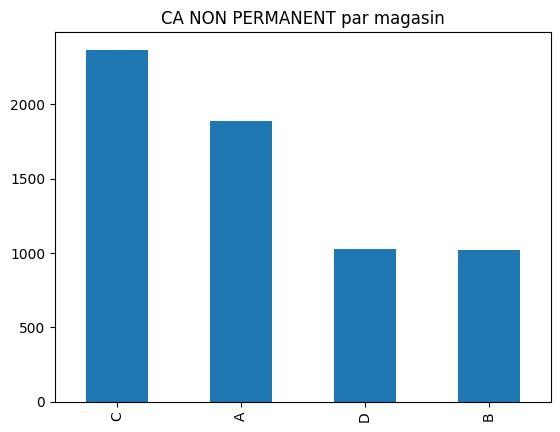
\includegraphics[height=3cm]{assets/__ca_non_permanent_par_magasin}
    \end{figure}
\end{frame}
